\documentclass[10pt,tgadventor, onlymath]{beamer}

\usepackage{graphicx,amsmath,amssymb,tikz,psfrag,neuralnetwork, fontawesome, xcolor}

%\input defs.tex
\graphicspath{ {./figures/} }
\input defs.tex

%% formatting

\mode<presentation>
{
\usetheme{default}
\usetheme{Berlin}

\usecolortheme{seahorse}
}
\setbeamertemplate{navigation symbols}{}
\usecolortheme[rgb={0.03,0.28,0.59}]{structure}
\setbeamertemplate{itemize subitem}{--}
\setbeamertemplate{frametitle} {
	\begin{center}
	  {\large\bf \insertframetitle}
	\end{center}
}

\newcommand\footlineon{
  \setbeamertemplate{footline} {
    \begin{beamercolorbox}[ht=2.5ex,dp=1.125ex,leftskip=.8cm,rightskip=.6cm]{structure}
      \footnotesize \insertsection
      \hfill
      {\insertframenumber}
    \end{beamercolorbox}
    \vskip 0.45cm
  }
}
\footlineon

\AtBeginSection[] 
{ 
	\begin{frame}<beamer> 
		\frametitle{Outline} 
		\tableofcontents[currentsection,currentsubsection] 
	\end{frame} 
} 


\tikzstyle{state}=[shape=circle,draw=blue!30,fill=blue!10]
\tikzstyle{observation}=[shape=rectangle,draw=orange!30,fill=orange!10]
\tikzstyle{lightedge}=[<-, dashed]
\tikzstyle{mainstate}=[state, thick]
\tikzstyle{mainedge}=[<-, thick]
\tikzstyle{block} = [draw,rectangle,thick,minimum height=2em,minimum width=2em]
\tikzstyle{sum} = [draw,circle,inner sep=0mm,minimum size=2mm]
\tikzstyle{connector} = [->,thick]
\tikzstyle{line} = [thick]
\tikzstyle{branch} = [circle,inner sep=0pt,minimum size=1mm,fill=black,draw=black]
\tikzstyle{guide} = []
\tikzstyle{snakeline} = [connector, decorate, decoration={pre length=0.2cm,
                         post length=0.2cm, snake, amplitude=.4mm,
                         segment length=2mm},thick, magenta, ->]



%% begin presentation

\title{\large \bfseries Asymptotic Capacity of Systems with Intelligent Reflective Surfaces}
\author{Peter Hartig \\ \and Supervisor: Saba Asaad}

\date{\today}

\begin{document}

\frame{
\thispagestyle{empty}
\titlepage
}

\section{Background}

\begin{frame}
\frametitle{Relaying}

	\begin{itemize}
		\item 			
			Base Stations Vs. Relay $\rightarrow$ reduced core network footprint/cost
%		\item 
%			Modes of operation provide cost/performance trade-off (decode and forward, amplify and forward ...)
		\item 
			Extending wireless coverage is relevant to high frequencies used in 5G +
	\end{itemize}

\end{frame}

\begin{frame}
\frametitle{Relay vs. Intelligent Reflective Surface}
\begin{columns}
\begin{column}{0.5\linewidth}
\centering 
	\underline{Relay: Amplify and Forward}
	\\
	\begin{equation*}
	\mathbf{y} = (\mathbf{H}_2\underbrace{\mathbf{F}}_{\text{Relay}}\mathbf{H}_1 + \underbrace{\mathbf{G}}_{\text{LOS}})\mathbf{x}
	\end{equation*}
	
	\begin{itemize}
	\item 
		$\mathbf{F}$ is diagonal
	\item 
		Requires expensive RF hardware
	\item 
		Can often ignore line of sight
	\item 
		Typically half-duplex
	\end{itemize}
\end{column}
\begin{column}{0.5\linewidth}
\centering 

	\underline{IRS}
	\\
	\begin{equation*}
	\mathbf{y} = (\mathbf{H}_2\underbrace{\boldsymbol{\Phi}}_{\text{IRS}}\mathbf{H}_1 + \underbrace{\mathbf{G}}_{\text{LOS}})\mathbf{x}
	\end{equation*} 
	\begin{itemize}
	\item 
		$\boldsymbol{\Phi}$ is diagonal with $| \phi_i | =1$
	\item 
		No RF chain required (low cost)
	\item
		Shorter distances $\rightarrow$ keep LOS
	\item 
		Inherently full-duplex
	\end{itemize}
\end{column}
\end{columns}

\end{frame}


%\begin{frame}
%\frametitle{IRS: Modes of Operation}
%\begin{columns}
%\begin{column}{0.5\linewidth}
%	Mode 1
%	\begin{figure}
%%			\centering
%		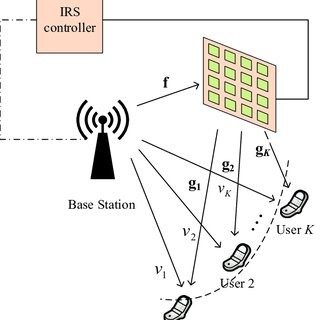
\includegraphics[scale=1]{irs}
%	\end{figure}\end{column}
%\begin{column}{0.5\linewidth}
%	Mode 2 (The one we will use)
%\end{column}
%\end{columns}
%\end{frame}
\begin{frame}
\frametitle{System Model}
\centering
\begin{equation*}
	\mathbf{y} = (\mathbf{H}_2\boldsymbol{\Phi}\mathbf{H}_1 + \mathbf{G})\mathbf{x}
\end{equation*}
with 
$\mathbf{H}_{1}\in \mathbb{C}_{S \times T},\mathbf{H}_{2} \in \mathbb{C}_{R \times S}, \mathbf{G} \in \mathbb{C}_{R \times T}$ and $\boldsymbol{\Phi}$ as $S \times S$ a diagonal matrix with $| \phi_i | =1$.

	\begin{figure}
		\centering
		\includegraphics[scale=.3]{irs_correct}
	\end{figure}
\end{frame}

\section{Goals}
\begin{frame}
\frametitle{Project Goals}
\begin{enumerate}
\item
	Find capacity of asymptotic IRS systems
	\begin{itemize}
	\item 
		Optimize phase matrix
	\item
		Generalize results
	\end{itemize}

\item 
	Confirm findings with numerical results throughout
	
\item
	* Time permitting - Consider secrecy capacity of IRS system
\end{enumerate}
\end{frame}

\section{Current Status}


\begin{frame}
\frametitle{Channel Capacity}
\begin{equation*}
	\mathbf{y} = (\mathbf{H}_2\boldsymbol{\Phi}\mathbf{H}_1 + \mathbf{G})\mathbf{x}
\end{equation*}

With $\mathbf{x}\mathbf{x}^H = \mathbf{I}$ and fixed $\boldsymbol{\Phi}$, capacity is given by 
\begin{equation*}\label{capacity}
\Expect\left[\Log\left(|\mathbf{I}_{R}+\frac{P_{\text{Total}}}{T \sigma_n}[\mathbf{H}_{2}\boldsymbol{\Phi}\mathbf{H}_{1} + \mathbf{G}][\mathbf{H}_{2}\boldsymbol{\Phi}\mathbf{H}_{1} + \mathbf{G}]^H|\right)\right].
\end{equation*}
Using 
\begin{equation*}
\mathbf{H}_{\text{Total}} = \mathbf{H}_{2}\boldsymbol{\Phi}\mathbf{H}_{1} + \mathbf{G}
\end{equation*}
and simplifying, \eqref{capacity} becomes
\begin{equation*}
N \int_0^{\infty}\Log\left(1+\frac{P_{\text{Total}}}{T \sigma_n} \lambda_{\mathbf{H}_{\text{Total}}\mathbf{H}_{\text{Total}}^H}\right) \textcolor{red}{p_{\lambda_{\mathbf{H}_{\text{Total}}\mathbf{H}_{\text{Total}}^H}}(\lambda)} d\lambda
\end{equation*}
with $N$ = rank($\mathbf{H}_{\text{Total}}$).
Need Asymptotic Eigenvalue Distribution (AED).
\end{frame}


\subsubsection{Previous Work + Free Probability}


\begin{frame}
\frametitle{Using Free Probability to find $p_{\lambda_{\mathbf{H}_{\text{Total}}\mathbf{H}_{\text{Total}}^H}}(\lambda)$}
Free probability provides a set of tools to find the AED of polynomials in free, self-adjoint operators (matrices).

\begin{itemize}
\item 
	For $\mathbf{A}$ and $\textbf{B}$ consider $\mathbf{C} = \mathbf{A} + \textbf{B}$ and $\mathbf{D} = \mathbf{A}\textbf{B}$
\item 
	Additive free convolution: $R_{\mathbf{C}}(w) = R_{\mathbf{A}}(w) + R_{\mathbf{B}}(w)$
\item 
	Multiplicative free convolution: $S_{\mathbf{D}}(z) = S_{\mathbf{A}}(z)S_{\mathbf{B}}(z)$
\end{itemize}

\begin{equation*}
\mathbf{H}_{\text{Total}}\mathbf{H}_{\text{Total}}^H 
= 
\underbrace{
\mathbf{H}_{2}\boldsymbol{\Phi}\mathbf{H}_{1}\mathbf{H}_{1}^H\boldsymbol{\Phi}^H\mathbf{H}_{2}^H +
\underbrace{\mathbf{H}_{2}\boldsymbol{\Phi}\mathbf{H}_{1}\mathbf{G}^H}_{\color{red}{\text{non-hermetian}}}+
\underbrace{\mathbf{G}\mathbf{H}_{1}^H\boldsymbol{\Phi}^H\mathbf{H}_{2}^H}_{\color{red}{\text{non-hermetian}}}+
\mathbf{G}\mathbf{G}^H
}_
{\color{red}{\text{not free}}}
\end{equation*}
%Need to show that these are not free!
\end{frame}

\begin{frame}
\frametitle{Free Probability}
The symmetrized density function.
\begin{equation*}
\tilde{p}(x) = \frac{p(x) + p(-x)}{2}
\end{equation*}
The symmetrized singular value, eigenvalue relationship.
\begin{equation*}\label{svd_aed_property}
\tilde{G}_{H}(s) = sG_{HH^{\dagger}}(s^2).
\end{equation*}
Additive free convolution still applies for singular values.
We only need the self-adjoint terms of the polynomial!
\end{frame}

\begin{frame}
\frametitle{Free Probability: Canceling Phase Terms}
Say 
\begin{equation*}
C_2 = \mathbf{H}_{2}\boldsymbol{\Phi}\mathbf{H}_{1}[\mathbf{H}_{2}\boldsymbol{\Phi}\mathbf{H}_{1}]^H
\end{equation*}
and a rotated version 
\begin{equation*}
\tilde{C}_2 = \underbrace{\boldsymbol{\Phi}^H\mathbf{H}_{2}^H\mathbf{H}_{2}\boldsymbol{\Phi}}_{C_{1}}\mathbf{H}_{1}\mathbf{H}_{1}^H.
\end{equation*}
Use the property 
\begin{equation*}\label{rotation_property}
S_{C_2}(z) = \frac{z+1}{z+\chi_2} S_{\tilde{C}_2}(\frac{z}{\chi_2}).
\end{equation*}
\pause
Repeat for
\begin{equation*}
C_{1} = \boldsymbol{\Phi}^H\mathbf{H}_{2}^H\mathbf{H}_{2}\boldsymbol{\Phi}
\end{equation*}
\begin{equation*}
\tilde{C}_{1} = \textcolor{red}{\boldsymbol{\Phi}\boldsymbol{\Phi}^H}\mathbf{H}_{2}^H\mathbf{H}_{2}
\end{equation*}
with $\boldsymbol{\Phi}\boldsymbol{\Phi}^H = \mathbf{I}$.
\end{frame}



\begin{frame}
	\frametitle{Capacity of constant channels with random phase
	}
	\centering 
	$\mathbf{H}_{2} \in \mathbb{C}_{R \times T}$, 
	$\mathbf{H}_{1} \in \mathbb{C}_{S \times T}$, with $\mathcal{CN}(0,\frac{1}{\sqrt{RS}})$
	and $ \mathbf{G} \in \mathbb{C}_{R \times T}$ with $\mathcal{CN}(0,\frac{1}{R})$. 
	Statistics from $1000$ random realizations of $\boldsymbol{\Phi}$.
	\bigskip
	
\begin{columns}
\begin{column}{0.5\linewidth}
\centering
Asymptotic case \\ $T = 100$, $ R = 100$ and $S = 100$
\begin{itemize}
\item
Capacity variance:
 0.0038458296727919886
 \item
Capacity average:
 6.764651253343401
 \item
Capacity min:
 6.574540172102809
 \item
Capacity max:
 6.98960781887363
\end{itemize}
%\textcolor{red}{\chi_N}}
\end{column}
\begin{column}{0.5\linewidth}
\centering
Non-asymptotic case\\ $T = R = 4$ and $S = 100$
\begin{itemize}
\item
Capacity variance:
 0.4157628312024758
 \item
Capacity average:
 4.014673474337778
 \item
Capacity min:
 2.146914646653352
 \item
Capacity max:
 6.130275960052021
\end{itemize}
\end{column}
\end{columns}
\end{frame}

\begin{frame}
	\frametitle{Numerical Results: Asymptotic Capacity}
	
	\begin{equation*}
	\mathbf{y} = (\mathbf{H}_2\underbrace{\boldsymbol{\Phi}}_{\text{IRS}}\mathbf{H}_1 + \underbrace{\mathbf{G}}_{\text{LOS: Rank $\leq 1$}})\mathbf{x}
	\end{equation*} 
\begin{figure}
\includegraphics[width= .75\linewidth, height = 5.5cm]{los}
\end{figure}
\end{frame}

\begin{frame}
	\frametitle{Numerical Results: Asymptotic Capacity}
		\begin{equation*}
	\mathbf{y} = (\underbrace{\sigma}_{\text{attenuation}}\mathbf{H}_2\underbrace{\boldsymbol{\Phi}}_{\text{IRS}}\mathbf{H}_1 + \underbrace{\mathbf{G}}_{\text{LOS}})\mathbf{x}
	\end{equation*} 
\begin{figure}
\includegraphics[width= .75\linewidth, height = 5.5cm]{attenuation}
\end{figure}
\end{frame}



\begin{frame}
\frametitle{Current Status}
\begin{enumerate}
\item
	Find capacity of asymptotic IRS systems  \faCheck
	\begin{itemize}
	\item 
		Optimize phase matrix	\faQuestion
	\item
		Generalize results
	\end{itemize}

\item 
	Confirm findings with numerical results throughout
	
\item
	* Time permitting - Consider secrecy capacity of IRS system
\end{enumerate}
\end{frame}


\section{Conclusion}

\begin{frame}
  \centering \Large
  \emph{Thank You.}
  \\
	\bigskip
    \centering \Large
  \emph{Questions or Comments?}

\end{frame}





\end{document}
